\section{observations}
In the experiment, the number of turns of the coil was $n=600$, average field line length for the sample $L=232$ mm, and $n/L= 2586.2$ m$^{-1}$. From the, we are able to calculate applied magnetic field intensity as,

\begin{align}
    H=(n/L)I
\end{align}

A observational values for the hysteresis curve and degaussing are given in tables I and II.
\begin{table*}
\begin{ruledtabular}
\begin{tabular}{|ccc|ccc|ccc|ccc|} 
     $I$ (A) & H (A/m) & B (Gauss) &  $I$ (A) & H (A/m) & B (Gauss) &  $I$ (A) & H (A/m) & B (Gauss) &  $I$ (A) & H (A/m) & B (Gauss) \\ \hline
     0.007 &   18.1  &   25 &  1.065 &  2754.31 &  2790 & -1.404 & -3631.03 & -2690 & 0.116 & 300.0  & -11 \\
     0.123 &  318.1  &  260 &  0.983 &  2542.24 &  2690 & -1.525 & -3943.97 & -2870 & 0.146 & 377.59  & 70  \\
     0.219 &  566.38 &  468 &  0.837 &  2164.66 &  2520 & -1.637 & -4233.62 & -3020 & 0.187 & 483.62  & 176 \\
     0.345 &  892.24 &  745 &  0.817 &  2112.93 &  2440 & -1.73  & -4474.14 & -3150 & 0.215 & 556.03  & 253 \\
     0.424 & 1096.55 &  935 &  0.779 &  2014.66 &  2380 & -1.806 & -4670.69 & -3240 & 0.28  & 724.14  & 424 \\
     0.522 & 1350    & 1171 &  0.694 &  1794.83 &  2230 & -1.941 & -5019.83 & -3400 & 0.37  & 956.9   & 670 \\
     0.632 & 1634.48 & 1429 &  0.605 &  1564.66 &  2070 & -1.985 & -5133.62 & -3450 & 0.445 & 1150.86 & 873 \\
     0.723 & 1869.83 & 1637 &  0.516 &  1334.48 &  1900 & -2.029 & -5247.41 & -3500 & 0.505 & 1306.03 & 1032\\
     0.807 & 2087.07 & 1822 &  0.4   &  1034.48 &  1630 & -1.906 & -4929.31 & -3420 & 0.622 & 1608.62 & 1340\\
     0.908 & 2348.28 & 2020 &  0.295 &   762.93 &  1376 & -1.805 & -4668.1  & -3350 & 0.699 & 1807.76 & 1528\\
     1.013 & 2619.83 & 2230 &  0.152 &   393.1  &   984 & -1.718 & -4443.1  & -3280 & 0.835 & 2159.48 & 1844\\
     1.18  & 3051.72 & 2530 &  0.074 &   191.38 &   782 & -1.55  & -4008.62 & -3150 & 0.955 & 2469.83 & 2100\\
     1.241 & 3209.48 & 2630 &  0.025 &    64.66 &   623 & -1.481 & -3830.17 & -3090 & 1  & 2586.21 & 2190\\
     1.303 & 3369.83 & 2750 & -0.013 &   -33.62 &   511 & -1.406 & -3636.21 & -3020 & 1.09  & 2818.97 & 2360\\
     1.4   & 3620.69 & 2880 & -0.121 &  -312.93 &   204 & -1.317 & -3406.03 & -2930 & 1.12  & 2896.55 & 2420\\
     1.527 & 3949.14 & 3050 & -0.197 &  -509.48 &   -13 & -1.202 & -3108.62 & -2800 & 1.285 & 3323.28 & 2710\\
     1.609 & 4161.21 & 3160 & -0.212 &  -548.28 &   -52 & -1.109 & -2868.1  & -2690 & 1.33  & 3439.66 & 2780\\
     1.736 & 4489.66 & 3320 & -0.274 &  -708.62 &  -222 & -1.021 & -2640.52 & -2580 & 1.372 & 3548.28 & 2850\\
     1.83  & 4732.76 & 3440 & -0.335 &  -866.38 &  -390 & -0.875 & -2262.93 & -2370 & 1.446 & 3739.66 & 2960\\
     1.937 & 5009.48 & 3560 & -0.427 & -1104.31 &  -638 & -0.782 & -2022.41 & -2220 & 1.49  & 3853.45 & 3020\\
     2.006 & 5187.93 & 3630 & -0.519 & -1342.24 &  -879 & -0.663 & -1714.66 & -2020 & 1.535 & 3969.83 & 3080\\
     1.9   & 4913.79 & 3570 & -0.642 & -1660.34 & -1189 & -0.574 & -1484.48 & -1856 & 1.609 & 4161.21 & 3180\\
     1.801 & 4657.76 & 3500 & -0.718 & -1856.9  & -1371 & -0.5   & -1293.1  & -1704 & 1.699 & 4393.97 & 3290\\
     1.689 & 4368.1  & 3420 & -0.81  & -2094.83 & -1584 & -0.396 & -1024.14 & -1470 & 1.743 & 4507.76 & 3350\\
     1.595 & 4125    & 3340 & -0.9   & -2327.59 & -1779 & -0.217 &  -561.21 & -1008 & 1.833 & 4740.52 & 3460\\
     1.52  & 3931.03 & 3270 & -1.022 & -2643.1  & -2020 & -0.114 &  -294.83 &  -710 & 1.906 & 4929.31 & 3540\\
     1.282 & 3315.52 & 3050 & -1.114 & -2881.03 & -2200 & -0.054 &  -139.66 &  -540 & 1.995 & 5159.48 & 3640\\
     1.203 & 3111.21 & 2960 & -1.221 & -3157.76 & -2390 & -0.01  &   -25.86 &  -408 &       &         &        \\
     1.155 & 2987.07 & 2900 & -1.312 & -3393.1  & -2545 &  0.011 &    28.45 &  -344 &       &         &        \\
    \end{tabular}  
\end{ruledtabular} 
\label{tab:1}
\caption{Data for the Hysteresis Curve}
\end{table*}
\begin{table}[H]
\centering
\begin{tabular}{|ccc|ccc|} \hline
    I & B & B$_r$ & I & B & B$_r$ \\ 
    (A) & (Gauss) &(Gauss) & (A) &(Gauss) & (Gauss) \\ \hline
    1.953 &  3620 &  581 & -0.945 & -1940 & -308 \\
    -23  & -3510 & -403 & 0.947  & 2130  & 493  \\
    -1.868 & -3360 & -410 & -0.828 & -1702 & -282 \\
     1.826 &  3480 &  580 & 0.834  & 1949  & 479  \\
    -1.708 & -3140 & -390 & -0.741 & -1512 & -263 \\
     1.711 &  3310 &  571 & 0.742  & 1715  & 448  \\
    -1.624 & -3050 & -389 & -0.622 & -1245 & -219 \\
     1.627 &  3230 &  569 & 0.624  & 1453  & 413  \\
    -1.508 & -2870 & -384 & -0.504 & -964  & -169 \\
     1.509 &  3050 &  560 & 0.505  & 1177  & 367  \\
    -1.42  & -2740 & -370 & -0.46  & -855  & -146 \\
     1.467 &  2990 &  556 & 0.415  & 958   & 321  \\
    -1.305 & -2570 & -359 & -0.37  & -640  & -98  \\
     1.308 &  2750 &  542 & 0.326  & 736   & 273  \\
    -1.22  & -2430 & -349 & -0.221 & -279  & 0    \\
     1.224 &  2620 &  533 & 0.221  & 492   & 203  \\
    -117 & -2120 & -328 & -0.131 & -76   & 72   \\
     18  &  2380 &  516 &        &         &        \\
    \hline
    \end{tabular}
    \label{tab:2}
\caption{Data from degaussing the iron core}
\end{table}

\section{Data Analysis and Calculations}

\subsection*{Hysteresis Curve}

From table I, we can plot the hysteresis curve for the iron core.

\begin{figure}[H]
    \centering
    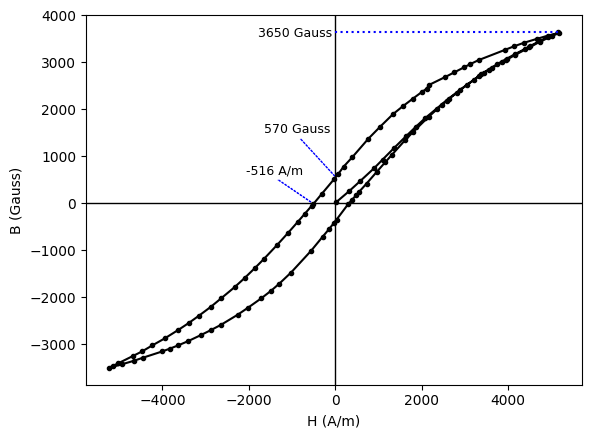
\includegraphics[width=1\columnwidth]{images/g1.png}
    \caption{Induced Magnetic field intensity ($B$) vs Applied Magnetic field intensity ($H$) curve}
    \label{graph:1}
\end{figure}

From Fig. \ref{graph:1}, we can find the the following parameters:

\begin{itemize}
    \item Saturation magnetization, by finding the saturation value of B, which is $B_S \approx 3650$ Gauss.
    \item Remanence or Retentivity, by finding $B|_{H=0} = B_r = 570$ Gauss.
    \item Coercivity, by finding $H|_{B=0} = H_C = 516$ A/m (in magnitude).
\end{itemize} 

\subsection*{Degaussing the Iron Core}
From table II, B vs $|$B$_r|$ plot was generated as follows.

\begin{figure}[H]
    \centering
    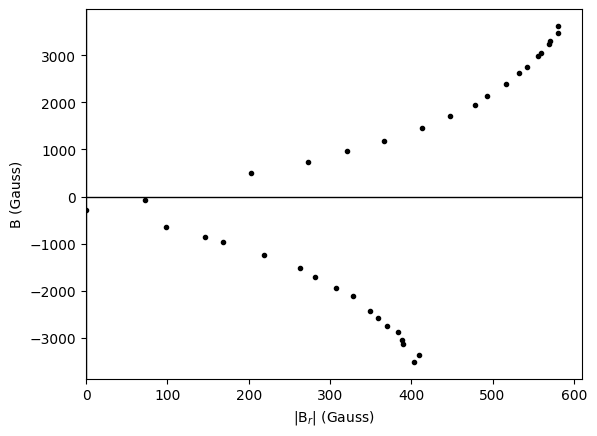
\includegraphics[width=1\columnwidth]{images/g2.png}
    \caption{Induced Magnetic field intensity ($B$) vs Magnitude of Remnant magnetic field at $I=0$ ($|B_r|$)}
    \label{graph:2}
\end{figure}

Here, we can see that the remnant magnetic field decreases and eventually reaches 0 as we continue degaussing the iron core.